\chapter{Miniprojekt}
\section{Opgavebeskrivelse}
Lav i Matlab en audio equalizer. Equalizeren skal kunne justere niveauet på et indkommende lydsignal i fem forskellige frekvensbånd (LP, BP1, BP2, BP3, HP fordelt over det hørbare spektrum) med +/- 12 dB. Equalizerens samlede impulsrespons og overføringskarakteristik (amplitude og fase i frekvensdomænet) skal kunne vises, og der skal laves to versioner: Én hvor filtreringen foregår i sample-domænet, og én som er baseret på multiplikation af de respektive komplekse frekvensspektre. Der skal i opgaven indgå filtre af begge typer (FIR og IIR).
\\ \\
Til test af denne audioequalizer er valgt en lydfil "musicex1", som er et jazzstykke, hvor de 10 første sekunder er udvalgt.
\section{Filtre}
Første step i designet af de fem forskellige filtre (LP, BP1, BP2, BP3 og HP), er at sætte knækfrekvenserne for de forskellige filtre. Knækfrekvenser er bestemt ud fra det hørebare spektrum, fra 80 Hz til 22kHz, hvor intervallet er fordelt ligeligt ud på hvert filter:
\begin{itemize}
	\item Lavpas
	\subitem Øvre = 4000
	\item Båndpas1
	\subitem Nedre = 3900
	\subitem Øvre = 8800 
	\item Båndpas2
	\subitem Nedre = 8700
	\subitem Øvre = 13200
	\item Båndpas3
	\subitem Nedre = 13100
	\subitem Øvre = 17600
	\item Højpas
	\subitem Nedre = 17500 
\end{itemize}

Desuden er der ved overgangen for hvert filter et overlap på 100 Hz, som sørger for at når filtreret knækker ikke mister lyden på nogle frekvenser eller får den forstærket yderligere. Grafisk vil dette vise en lige linje når alle filtre summeret sammen i samme figur. Se figur \ref{Figur 1} \\
Filtrene designes som enten FIR filter med en orden = 1000, ved fir1 funktionen, eller som IIR filter med orden = 6, ved butter (butterworth filter) funktionen.
\begin{figure}[H]
	\centering
	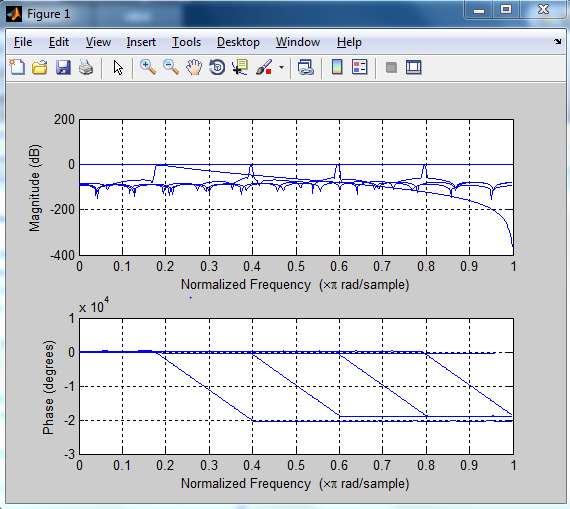
\includegraphics[width=0.8\textwidth]{Figurer/Figur_1}
	\caption{Summerede filtre}
	\label{Figur 1}
\end{figure}

\section{Filtrering}
Først plottes det ufiltrerede signal(figur \ref{Figur 2}), for senere at kunne sammenligne med det filtrerede signal (figur \ref{figur 3}):

\begin{figure}[H]
	\centering
	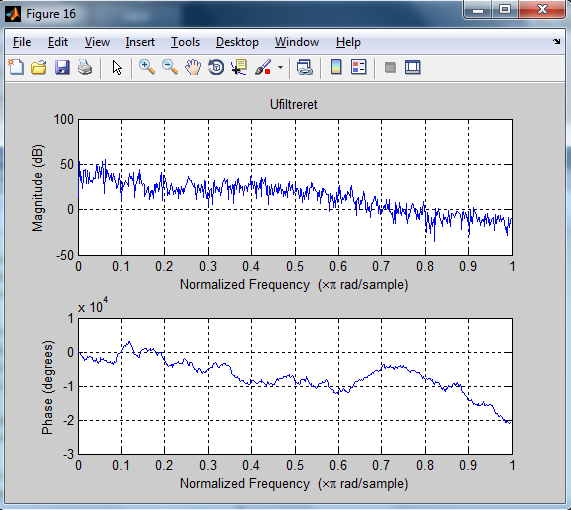
\includegraphics[width=0.8\textwidth]{Figurer/Ufiltreret_signal}
	\caption{Ufiltreret signal}
	\label{Figur 2}
\end{figure}

\begin{figure}[H]
	\centering
	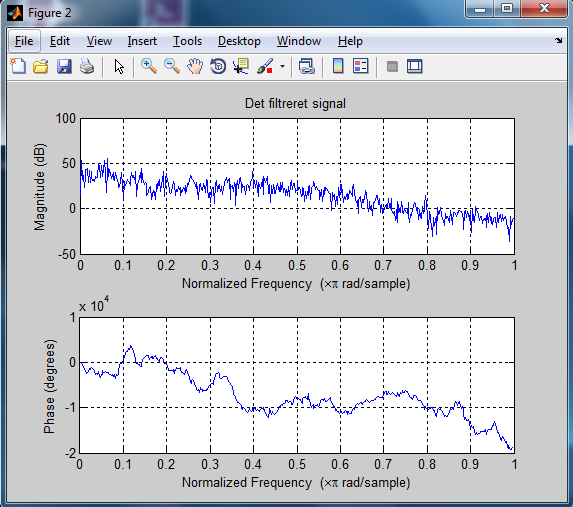
\includegraphics[width=0.8\textwidth]{Figurer/2_Filtreret_signal}
	\caption{Filtreret signal}
	\label{figur 3}
\end{figure}
Når signalet er kørt gennem alle filtrene uden forstærkning, ses det at signalet er uændret. Ved ændring af forstærkningskoefficienterne vil signalet ændres. Nedenfor på figur \ref{Figur 4} ses et signal, hvor båndpas1 er ganget med en faktor 50 og båndpas2 er ganget med en faktor 0.1:

\begin{figure}[h]
	\centering
	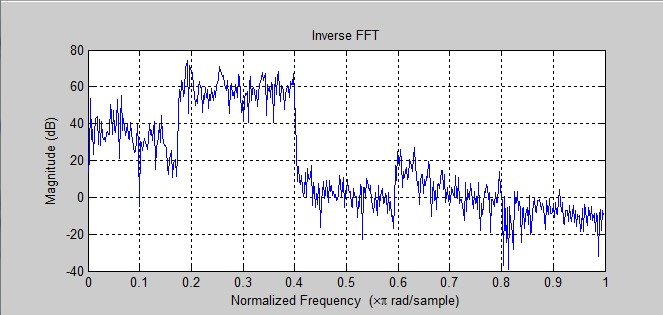
\includegraphics[width=0.8\textwidth]{Figurer/Forstaerkning_og_Daempning}
	\caption{Manipuleret signal}
	\label{figur 4}
\end{figure}

\section{FFT af filtre}
\subsection{Lavpas}
Der er her foretaget FFT (Fast Fourier Transformation), i første omgang FFT af input signalet, hvorefter impulsresponens kan findes ved impz funktionen (figur \ref{Figur 5}:

\begin{figure}[h]
	\centering
	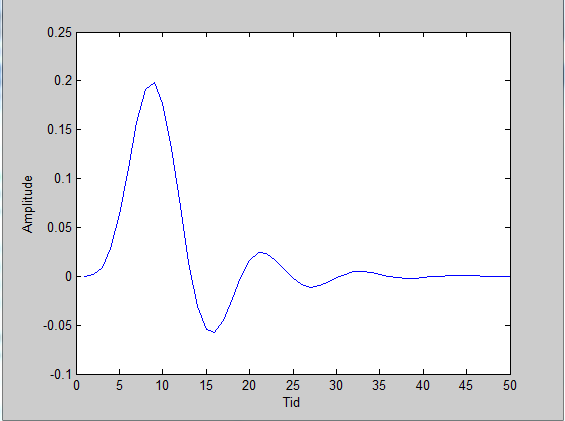
\includegraphics[width=0.8\textwidth]{Figurer/FFT_IIR}
	\caption{Impulsrespons}
	\label{Figur 5}
\end{figure}

Ud fraimpulsresponses laves FFT af det IIR lavpas filtrerede signal, først amplitudespektret (figur \ref{Figur 6}), hvor det ses hvilke at de lave frekvenser lukkes igennem:

\begin{figure}[h]
	\centering
	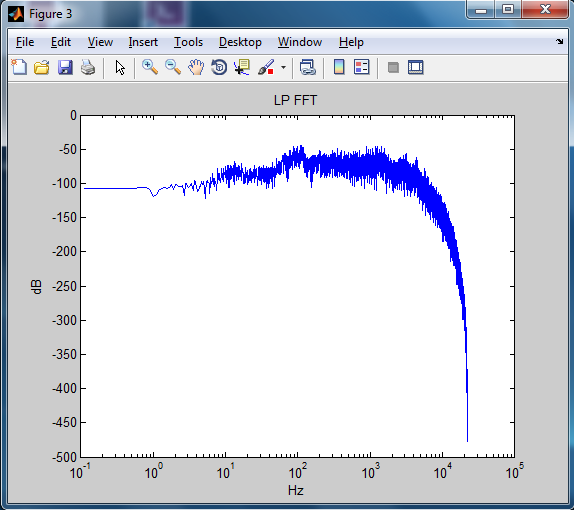
\includegraphics[width=0.8\textwidth]{Figurer/3_LP_FFT}
	\caption{Amplitude IIR lavpas FFT}
	\label{Figur 6}
\end{figure}

\subsection{Båndpasfiltre}
Ved FIR filtrene er det ikke nødvendigt at finde impulseresponsen.

\begin{figure}[h]
	\centering
	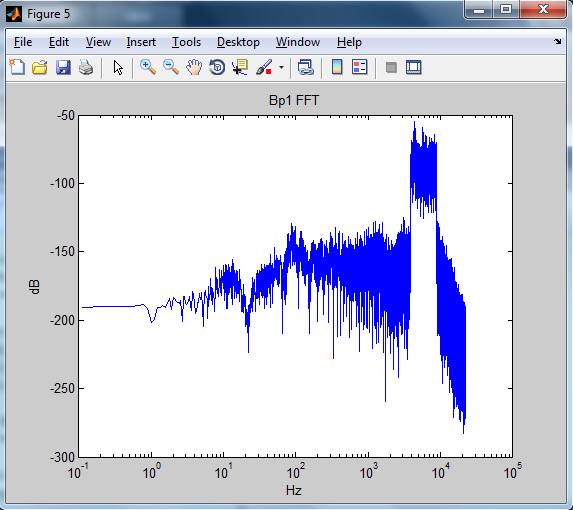
\includegraphics[width=0.8\textwidth]{Figurer/4_Bp1_FFT}
	\caption{FFT båndpas 1}
	\label{Figur 7}
\end{figure}

\begin{figure}[h]
	\centering
	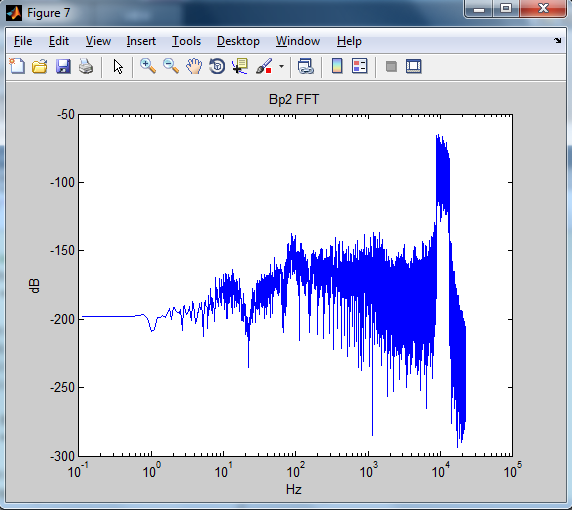
\includegraphics[width=0.8\textwidth]{Figurer/5_Bp2_FFT}
	\caption{FFT båndpas 2}
	\label{Figur 8}
\end{figure}

\begin{figure}[h]
	\centering
	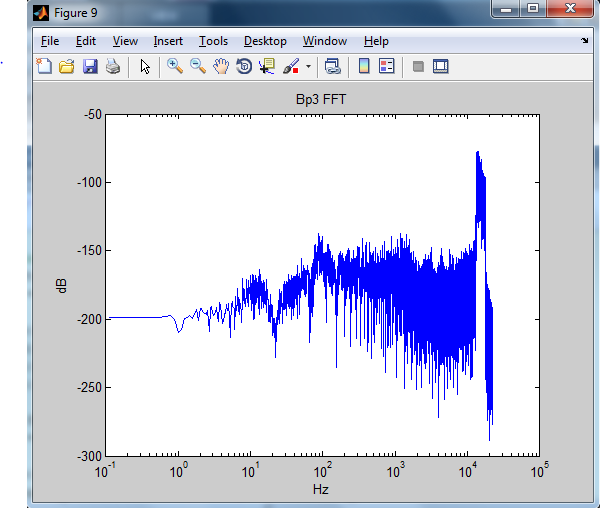
\includegraphics[width=0.8\textwidth]{Figurer/6_Bp3_FFT}
	\caption{FFT båndpas 3}
	\label{Figur 9}
\end{figure}

Ved båndpas filtrene ses en forstærkning som stemmer overens med knækfrekvenserne, derfor sker forstærkningen ved forskellige Hz i båndpas1, 2 og 3.

\subsection{Højpas}
Højpasfilter er lavet på samme måde som de andre FIR filtre, uden en øvre knækfrekvens:
\begin{figure}[h]
	\centering
	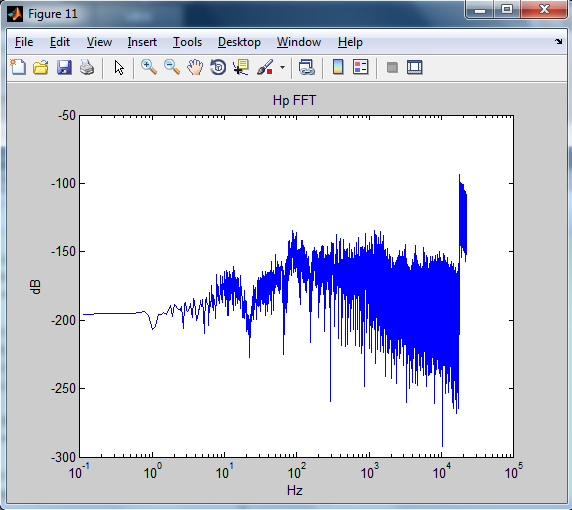
\includegraphics[width=0.8\textwidth]{Figurer/7_HP_FFT}
	\caption{FFT højpas}
	\label{Figur 10}
\end{figure}

\subsection{Summeret signal}
For at finde et samlet FFT signal, altså det samlede output, summeres alle FFT signalerne (figur \ref{Figur 11}:

\begin{figure}[h]
	\centering
	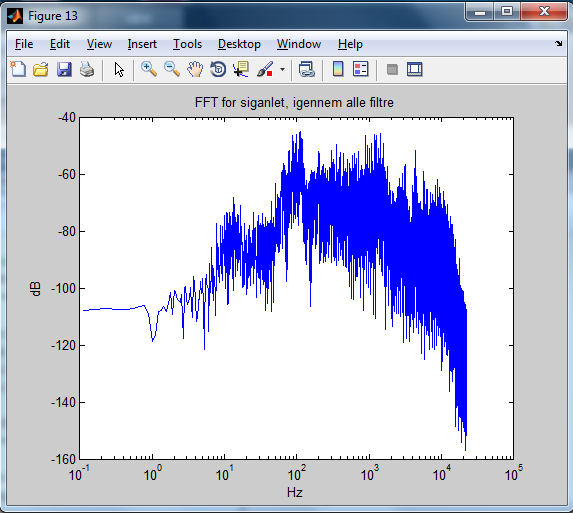
\includegraphics[width=0.8\textwidth]{Figurer/8_FFT_signalet_Alle_Filtre}
	\caption{FFT samlet}
	\label{Figur 11}
\end{figure}

Det er den inverse FFT af ovenstående signal der skal bruges til sammenligning af det ufiltrerede signal, og signalet der har været gennem alle filtre. Det inverse FFT af signal ses på figur \ref{Figur 12}:

\begin{figure}[h]
	\centering
	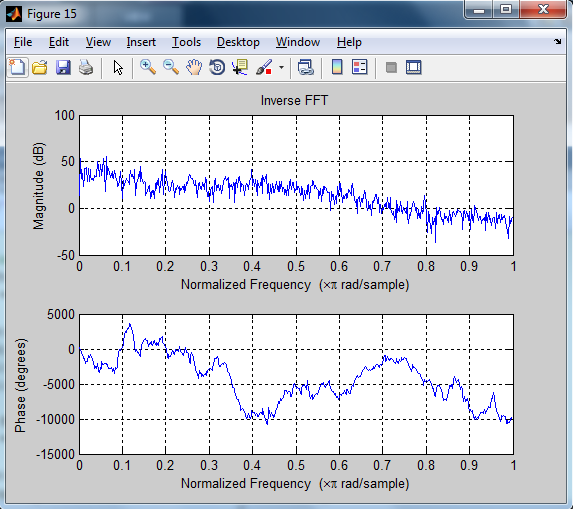
\includegraphics[width=0.8\textwidth]{Figurer/Invers_FFT_Hele_signalet}
	\caption{Invers FFT}
	\label{Figur 12}
\end{figure}

\begin{figure}[h]
	\centering
	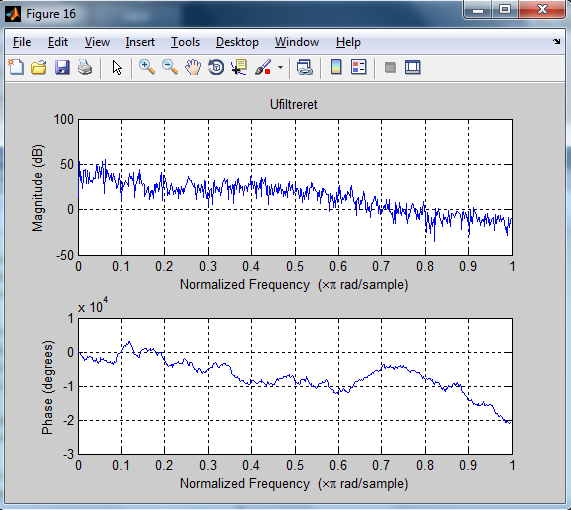
\includegraphics[width=0.8\textwidth]{Figurer/Ufiltreret_signal}
	\caption{Ufiltreret signal}
	\label{Figur 2}
\end{figure}

\begin{figure}[h]
	\centering
	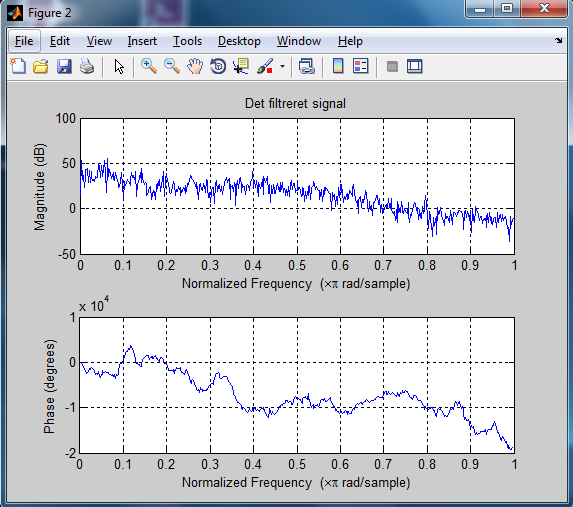
\includegraphics[width=0.8\textwidth]{Figurer/2_Filtreret_signal}
	\caption{Filtreret signal}
	\label{figur 3}
\end{figure}


Det ses at både det inverse FFT signal, det ufiltrerede signal og det filtrerede singal stemmer overens. Dette lever også op til det forventede, da de summerede filtre udgør en stort set ret linje, og dermed ikke forstærker eller dæmper signalet.


